%!TEX encoding = IsoLatin

\documentclass[12pt]{ULrapport}
\usepackage[ansinew]{inputenc}
\usepackage[french]{babel}
\usepackage{float}
\restylefloat{table}
\usepackage{hhline}
\usepackage{pdfpages}
\usepackage{hyperref}
\usepackage{multirow}


% Title Page
\title{Design III: Pirates des Cara�bes}
\author{S�bastien Garvin, Xavier Kedzierski, Matthieu Sylvain, J�r�my Brown, Charles-Olivier Magnan, Jean-Michel Provencher}



\TitreProjet{Design III}                       
\TitreRapport{Remise 3}                      
\Destinataire{Philippe Gigu�re, Dominique Grenier, Denis Laurendeau}         
\NumeroEquipe{7}                                     
\NomEquipe{Zi�re}                               
\TableauMembres{%
	111\,114\,478  & Garvin, S�bastien   & \\\hline 
	111\,040\,128  & Kedzierski, Xavier   & \\\hline     
	111\,066\,466  & Magnan, Charles-Olivier      & \\\hline
	111\,071\,384  & Provencher, Jean-Michel   & \\\hline     
	111\,073\,630	 & Bourque, Emile						& \\\hline
	111\,075\,478	 & Sylvain, Matthieu			& \\\hline
	111\,074\,361  & Brown, J�r�my				& \\\hline
	907\,196\,009  & Garneau, Laurent			& \\\hline
}
\DateRemise{3 avril 2016} 
% Contenu de l'historique des versions
\HistoriqueVersions{%										% version & date & description \\\hline
       1.0  & 24 janvier 2016 & Cr�ation du document \\\hline
			 2.0  & 31 janvier 2016 & Remise 1 \\\hline
			 3.0  & 28 f�vrier 2016 & Remise 2 \\\hline
			 4.0  & 3 avril 2016    & Remise 3 \\\hline
			}

\begin{document}

% Chapitres
\chapter{Diagrammes}
\label{s:Diagrammes}


\section{Diagramme de contexte}
\label{s:Diagramme_contexte}

\begin{figure}[htp]
   \centering
   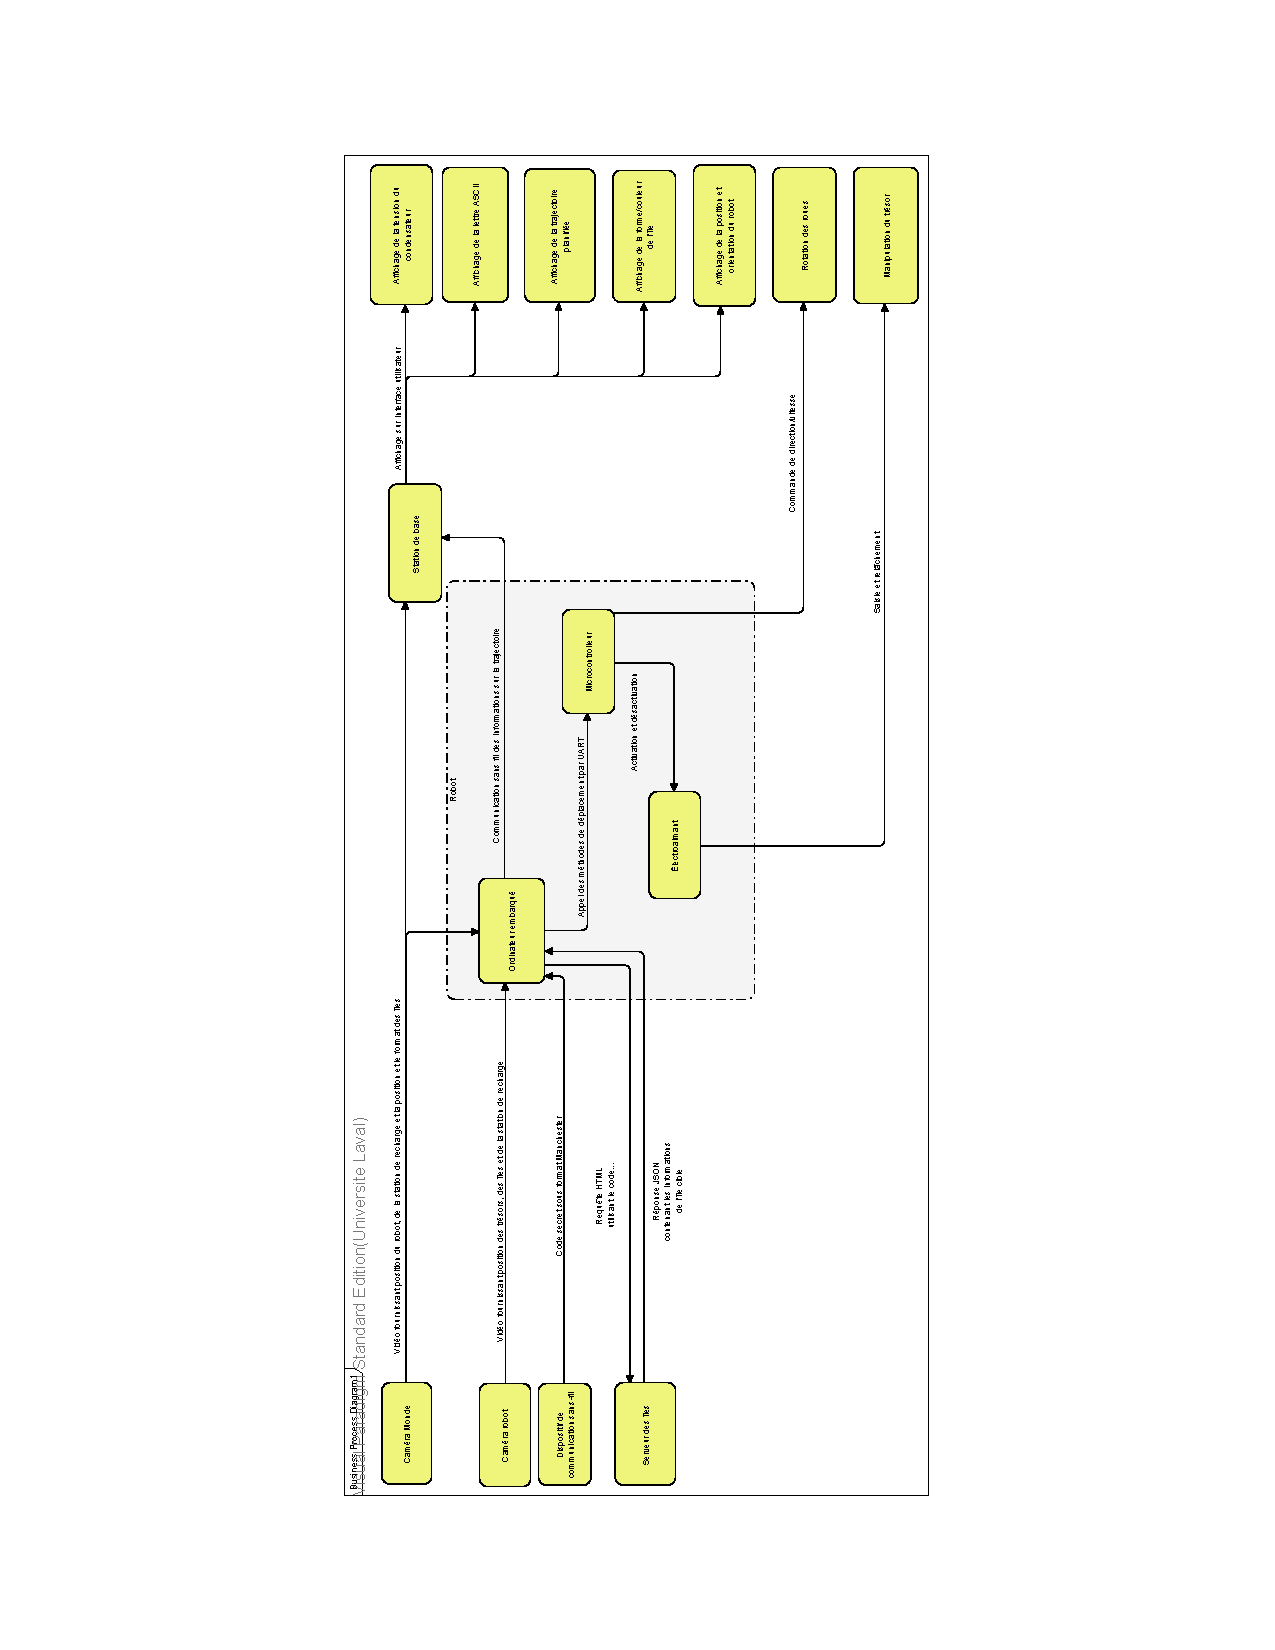
\includegraphics[width=0.75\textwidth, angle =-90]{pdf/ContextDiagram.pdf}
   \caption{Diagramme de contexte}
   \label{f:Diagramme_contexte}
\end{figure}

\newpage

\section{Diagramme de classes}
\label{s:Diagramme_classes}

\begin{figure}[htp]
   \centering
   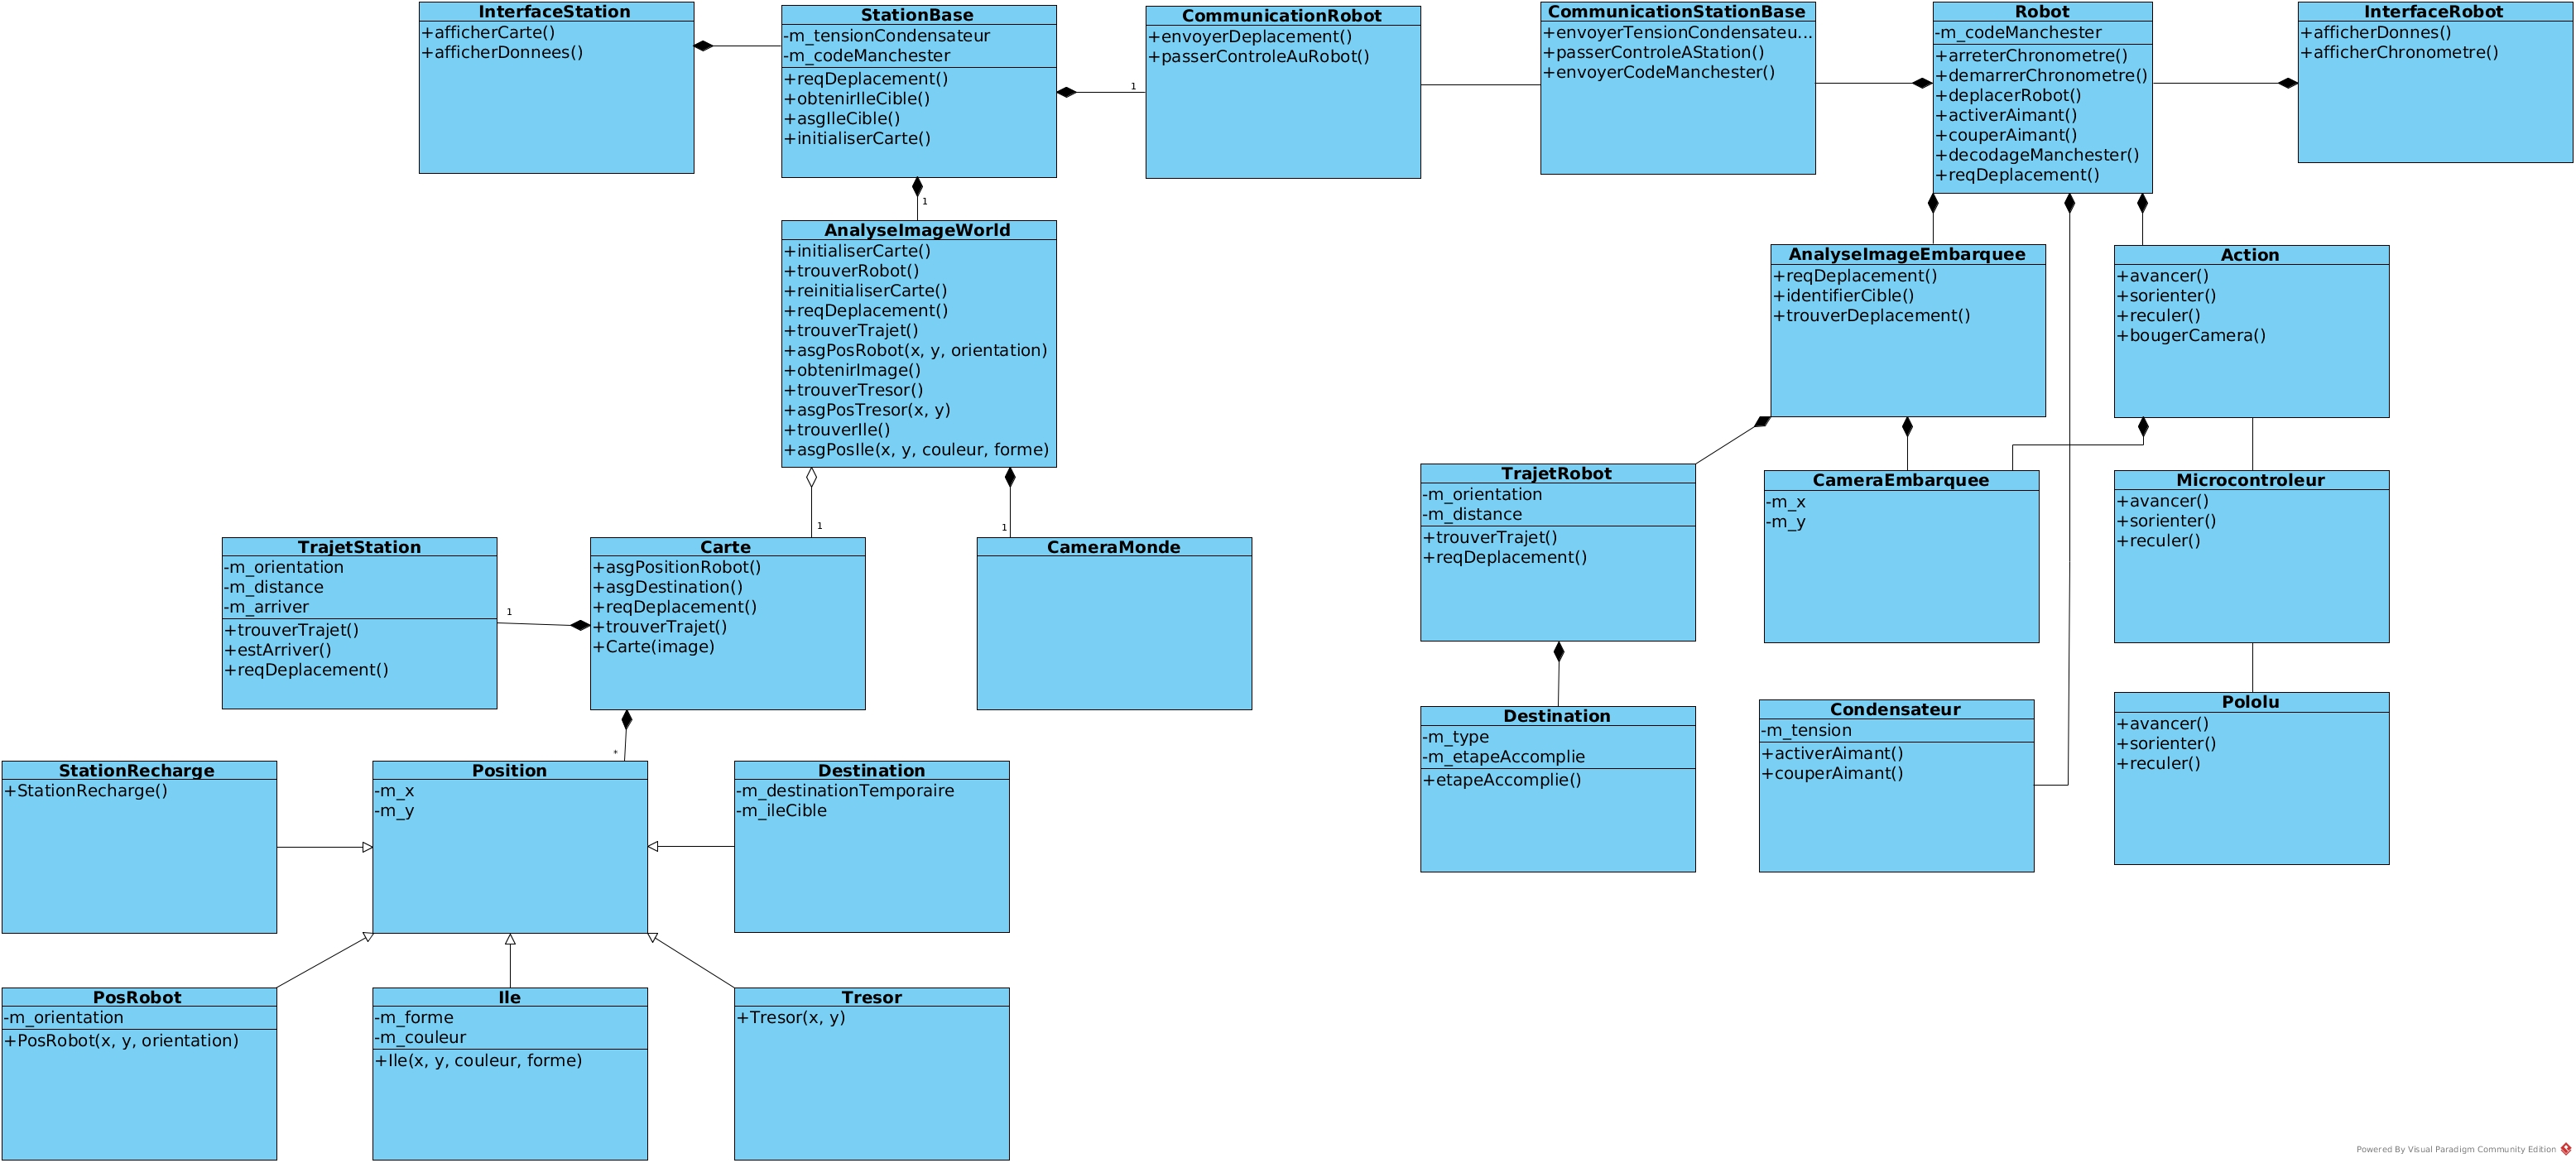
\includegraphics[width=0.95\textwidth, angle =-90]{fig/ClassDiagram.jpg}
   \caption{Diagramme de classes}
   \label{f:Diagramme_Classes}
\end{figure}

\newpage


La figure \ref{f:Diagramme_Classes} repr�sente le diagramme de classes suite � la premi�re it�ration. La structure est suseptible de changer suite aux prochaine it�rations, mais voici une br�ve description de la structure sur laquelle nous nous entendons pr�sentement. \par

La section de gauche du diagramme sera impl�ment�e sur la station de base tandis que la section droite sera impl�ment�e sur le robot. Ces deux syst�me pouront communiquer entre eux � l'aide des classes CommunicationRobot et CommunicationStationBase. \par

En ce qui conscerne la station de base, le contr�leur du syst�me est repr�sent� par la classe StationBase. La classe AnalyseImageWorld analyse les images re�u de la CameraMonde et g�n�re une carte sh�matique de la table (Carte) � l'aide d'imagerie. La carte est compos�e de diverses �l�ments qui h�rite tous de la classe Position. Les trajectoires du robot seront calcul� dans la classe TrajetStation � l'aide des informations de la classe Carte.  \par

Pour ce qui est du robot, il est aussi compos� d'un contr�leur (Robot). Les mouvements que devra effectuer le robot passerons tous par la classe Action qui les acheminera au microcontroleur et au polulu si nescessaire. Lorsque le robot est pr�s de la destination, TrajetRobot calculera les trajets (� l'aide de Destination et d'imagerie effectu� dans AnalyseImageEmbarquer).

    
   



\section{Diagramme de s�quences}
\label{s:Diagramme_sequences}

\begin{figure}[htp]
	\centering
	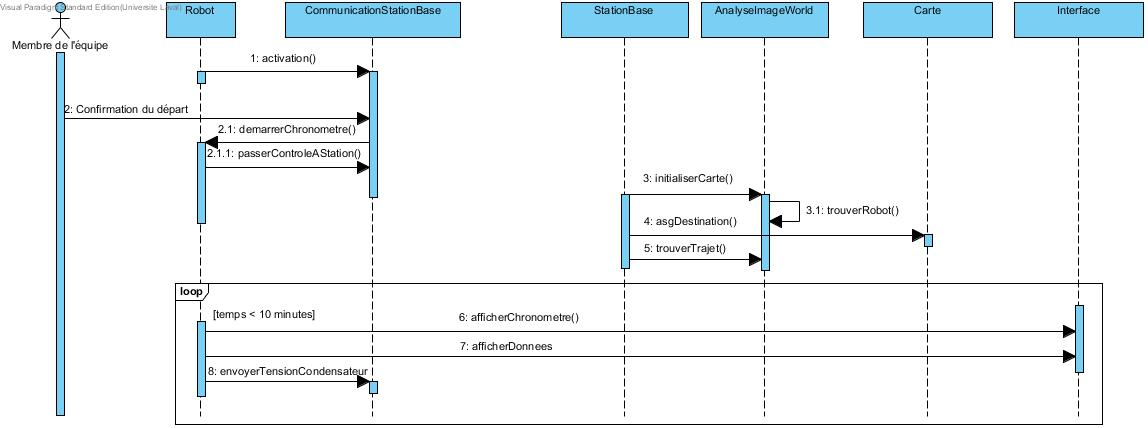
\includegraphics[width=0.95\textwidth]{fig/demarrageRobot.jpg}
	\caption{D�marrage du Robot}
	\label{f:DemRob}
\end{figure}

%\begin{figure}[htp]
%   \centering
%   \includegraphics[width=1\textwidth]{Diagramme_sequences}
%   \caption{Diagramme de s�quences}
%   \label{f:Diagramme_sequences}
%\end{figure}


\chapter{Plan d'int�gration}
\label{s:PlanIntegration}


\begin{figure}[htp]
   \centering
   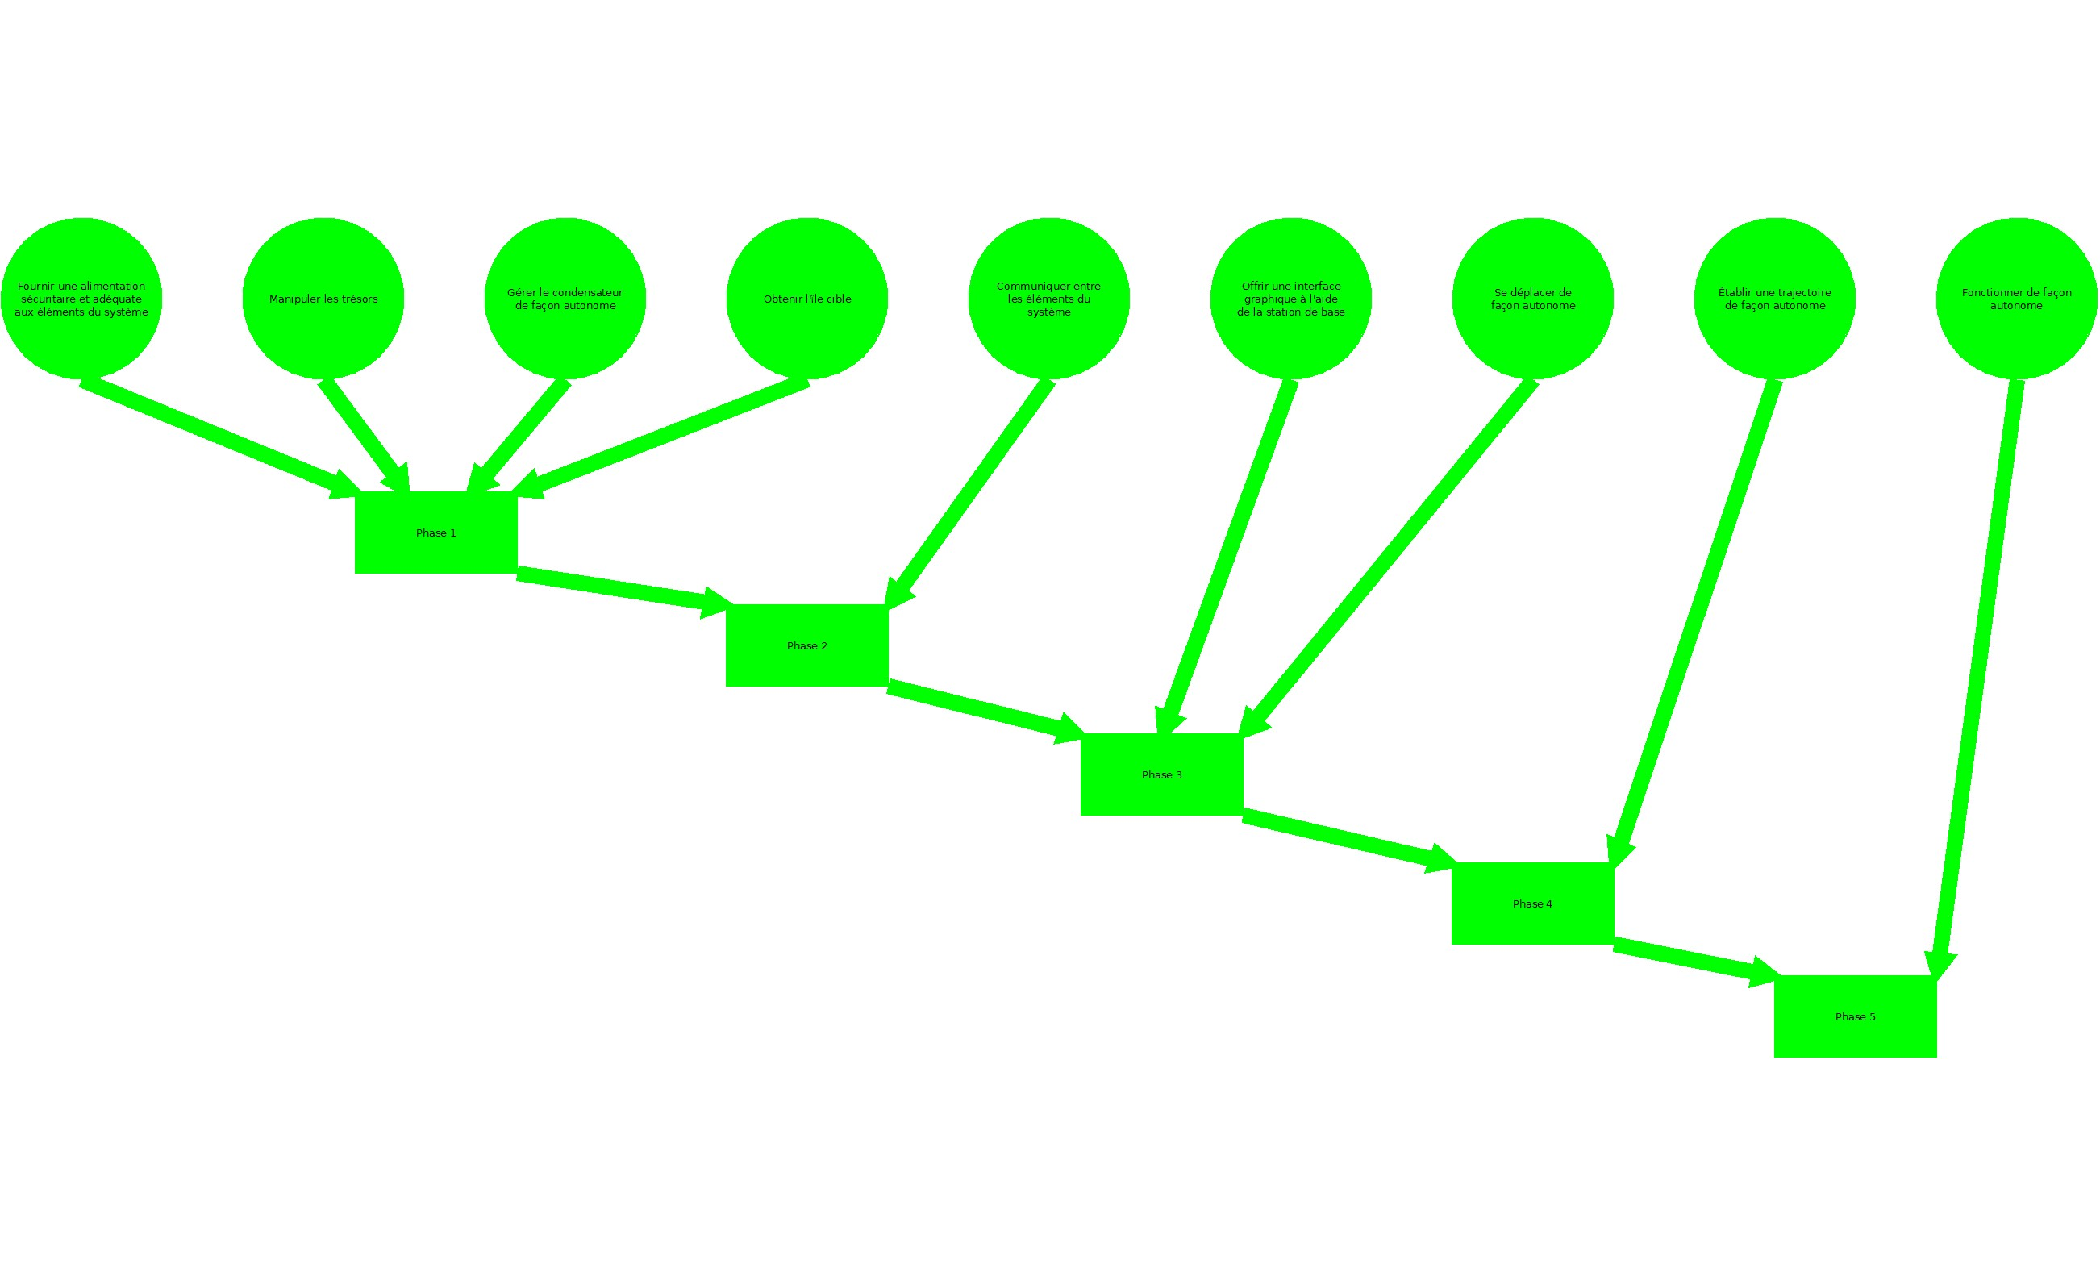
\includegraphics[width=1\textwidth]{pdf/PlanIntegration.pdf}
   \caption{Plan d'int�gration}
   \label{f:plan_integration}
\end{figure}



\chapter{Vision}
\label{s:Vision}



%

\section{Diagramme de classe}

Puisque la taille du diagramme de classe est tr�s grande, celui-ci peut �tre retrouv� � l'int�rieur du dossier /fig inclut avec la remise. Une br�ve description du flot d'ex�cution de la routine suivra afin de mieux comprendre l'utilit� des classes principales.
\medbreak

Du c�t� de la station de base, l'interface est d'abord initialis�e par le main. Ensuite, les boutons peuvent �tre utilis�s afin de d�marrer une certaine routine en initialisant la classe StationBase avec la table de jeux utilis�e et la routine voulue. Ce thread est le contr�leur de la station et est celui qui initialise par la suite les threads suivants: 
\begin{enumerate}
\item \textbf{StationServeur :} Initialise une connexion TCP avec le robot (avec TCPServeur). Il est en charge d'envoyer et de traiter toute communication entre la station de base et le robot. La communication est effectu�e sous forme d'envoie de fichier JSON qui sont cr��s par la classe RequeteJSON.
\item \textbf{FeedVideoStation :} Ce thread ne fait que lire les images de la cam�ra world afin qu'elles soient analys�es par la suite.
\item \textbf{AnalyseImageWorld :} Rep�re les iles, les tr�sors et le robot avec l'aide de plusieurs classes de d�tection. Pour la d�tection des �l�ments, les intervalles de couleur sont celles correspondantes � la table actuelle d�finit lors de l'initialisation de la station de base. Une fois trouv�s, tous les �l�ments cartographiques sont ajout� � la classe Carte.
\item \textbf{ImageVirtuelle :} Ce thread est en charge de dessiner sur l'image obtenue, afin de l'afficher dans l'interface. Les informations telles que la trajectoire pr�vue, la position r�elle du robot et les autres �l�ments cartographiques d�tect�s. Cette classe repr�sente donc tout simplement la carte virtuelle.
\end{enumerate}
Suite � l'initialisation de StationBase, Interface initialise un dernier thread (AfficherImageVirtuelle). Celui-ci ne fait que mettre � jour le feed vid�o (ImageVirtuelle) dans l'interface.  
\medbreak
D�s le d�but de l'ex�cution, la classe StationBase initialise la classe Trajectoire avec GrilleCellule. Celle-ci repr�sente la matrice de position o� le robot peut �tre positionn�. Lors de la demande d'un trajet, Trajectoire appelle AlgorithmeTrajectoire avec la grille de cellule. Cette classe trouvera la trajectoire demand�e selon le contenu des cellules. 
\medbreak
Finalement, la classe RedirigeurTexte sert tout simplement � rediriger les impressions consoles dans la boite de texte de l'interface.\bigbreak
Du cot� du robot, le contr�leur est la classe Robot. La communication se d�roule comme avec la station de base avec les classes (RequeteJSON, RobotClient, TCPClient). La classe UARTDriver est utilis�e pour envoyer des commandes par UART, tandis que la classe LectureUART est utilis�e pour lire et traiter les donn�es envoy�es par le UART.
\medbreak
Lorsque le robot entre en phase d'alignement, il se sert de AnalyseImageEmbarquee et de la classe de d�tection correspondante afin de trouver les ajustements requis. Les ajustements sont ensuite transmis au robot et sont envoy�es au UART afin de terminer la phase d'alignement.
\medbreak
La classe RobotService est utilis�e pour effectuer du traitement d'information. Elle est utilis�e pour effectuer la requ�te au serveur des iles, gr�ce au code Manchester pr�alablement d�cod�. Ensuite, elle traite la r�ponse pour obtenir l'indice sur l'ile cible.
\bigbreak
Finalement, la classe ConfigPath est utilis�e afin de transformer les adresses locales en adresses absolues. 

%Les sections \ref{locIle} et \ref{locRobot} se d�roulent �videmment sur la station de base. Il est a noter que lors de la r�ception d'une nouvelle image, celle-ci commence par la redimensionner de sorte � ne contenir que la table. Par la suite, un Gaussian blur est effectu�. C'est � ce stade que les d�tections sont effectu�e. 

 \section{Localisation des iles et des tr�sors}
\label{locIle}
Le processus de localisation des �les est effectu�, au tout d�but de la routine. Pour localiser les �les, chacune des quatre couleurs est filtr�e et plac�e dans un masque afin d'effectuer un traitement individuel. Ensuite, les formes ayant une aire trop grande ou trop petite sont �limin�es. Par la suite, les formes poss�dant un trou (contour enfant) avec un aire consid�rable sont �limin�es (voir \ref{locRobot}). Le syst�me compare ensuite les contours restant des formes filtr�es avec les formes g�om�triques en m�moire. De ce fait, celui-ci est en mesure d'identifier la forme qui poss�de le plus haut taux de compatibilit� avec celles en m�moire. Si l'indice de pr�cision est trop faible pour les quatre formes en m�moire, la forme est ignor�e. Bien que ce processus soit d�j� robuste, ceci est effectu�e � dix reprises dans le but de conserver la liste d'�le ayant la longueur la plus constante.
 \medbreak
Pour ce qui est de la localisation des tr�sors, un processus similaire est utilis�. L'image est filtr�e (� dix reprises) avec la couleur des tr�sors, puis les formes d�tect�es sont retenues ou non d�pendamment de l'aire de celles-ci. Les formes des tr�sors ne sont donc pas compar�es, mais les tr�sors ne se retrouvant pas sur le long des murs sont n�glig�s. Cette derni�re op�ration s'effectue facilement puisque l'image est redimensionn�e de sorte � ne contenir que la table avant la d�tection.
 
 
 \section{Localisation du robot}

\label{locRobot}
Puisque la d�tection des �les se d�roule avec succ�s, la m�me base est appliqu�e au robot. En effet, sur le dessus de celui-ci se retrouvent deux formes (carr� et cercle) de la m�me couleur situ�e sur le m�me axe. Par contre, afin de les diff�rencier des �les, elles poss�dent un trou blanc � l'int�rieur (voir figure \ref{f:detectRobot}). L'image redimentionn�e de la table est donc filtr�e avec la couleur du robot et plac�e dans un masque. Ensuite (comme pour les �les), les formes ayant une aire trop grande ou trop petite sont �limin�es. Par la suite, les formes ne poss�dant pas un trou (contour enfant) avec une aire consid�rable sont �limin�es. Le syst�me compare ensuite les contours restant avec les formes g�om�triques en m�moire. De ce fait, celui-ci est en mesure d'identifier la forme qui poss�de le plus haut taux de compatibilit� avec celles en m�moire. Si l'indice de pr�cision est trop faible pour les deux formes en m�moire, le robot ne sera pas d�tect� � cette it�ration. \medbreak
\begin{figure}[htp]
   \centering
   
\includegraphics[width=0.5\textwidth]{fig/imageRobot.png}
   \caption{Image de la forme sur le robot}
   \label{f:detectRobot}
\end{figure}
Une fois les contours d�tect�s, un peu de g�om�trie permet d'obtenir les donn�es voulues. Les formes sont positionn�es de sorte que le centre des deux formes est situ� au centre du robot. L'orientation du robot est simplement l'orientation du vecteur reliant le centre des deux formes (sachant que le cercle est l'avant du robot). \medbreak
Afin d'ajouter un peu de robustesse � ce proc�d�, les d�tections subs�quentes consid�rent l'ancienne position du robot et une analyse de faisabilit� du d�placement est effectu�e. Si le d�placement est trop �lev�, le robot n'est pas d�tect�. Dans l'�ventualit� o� le robot n'est pas d�tect� lors de dix it�rations cons�cutives, le robot est d�clar� comme perdu et l'analyse de faisabilit� de d�placement est ignor�e jusqu'� ce qu'il soit retrouv�.

\section{Phases d'alignement du robot}
Tout d'abord, il est important de sp�cifier que la station de base g�re les d�placements principaux du robot alors que le robot g�re lui-m�me les phases d'alignements. Ceci dit, lorsque le robot est dirig� vers une position cible, la station de base lui indiquera quelle type d'alignement il doit effectuer. Il y a une phase d'alignement unique pour la capture d'un tr�sor, le d�p�t de celui-ci sur l'�le cible ainsi que pour l'amarrage du robot avec la station de recharge.
\medbreak
Les phases d'alignement regroupent plusieurs petites �tapes. Tout commence avec le changement de l'orientation de la cam�ra embarqu�e. Celle-ci poss�de plusieurs positions pr�d�finies, ce qui facilite grandement le d�roulement du processus d'alignement.

\subsection{Capture du tr�sor}
Pour la capture du tr�sor, la cam�ra est plac�e en "position tr�sor" afin d'identifier le tr�sor et �valuer la distance le s�parant du robot. La distance est obtenue en comparant la dimension du tr�sor avec une dimension de r�f�rence �tablie lors de la phase de test. 
\medbreak
Ensuite, puisque la position du pr�henseur sur le robot est connue, le robot calcule les ajustements n�cessaires et les commandes appropri�es sont calcul�es. Une fois la commande de d�placement lat�ral effectu�e, l'�lectroaimant est activ� et le pr�henseur est abaiss�. Le robot effectue par la suite un d�placement frontal, capture le tr�sor, remonte le pr�henseur et recule afin de valider que le tr�sor a bel et bien �t� captur� en effectuant une autre analyse d'image. La phase de pr�hension de tr�sor se termine donc et la station de base reprendra le contr�le du robot.  

\subsection{D�p�t du tr�sor}
Pour le d�p�t du tr�sor, la cam�ra se positionne face � la surface de jeu et analyse la position de l'�le cible pour calculer le d�placement vertical et horizontal � effectuer. Une fois ces ajustements calcul�s, des commandes de d�placements sont envoy�s. Finalement, une fois l'alignement termin�, le syst�me valide la position de l'�le cible par rapport � la zone de d�p�t s�curitaire d�termin�e par des tests. Le tr�sor est soit d�pos� ou un autre alignement est effectu�. Pour d�poser le tr�sor, l'�lectroaimant est activ�, puis le pr�henseur est abaiss� en douceur. Une fois le pr�henseur abaiss�, l'�lectroaimant est d�sactiv� et quelques secondes plus tard, le pr�henseur remonte.
\medbreak
Un exemple de l'analyse effectu�e par le syst�me lors de la phase d'alignement avec l'ile cible peut �tre observ� � la figure \ref{f:alignement_ile}. Le syst�me calcule les ajustements n�cessaires afin que le centre de l'ile se trouve dans la zone de d�p�t s�curitaire une fois ces ajustements effectu�s par le robot.
\begin{figure}[htp]
   \centering
   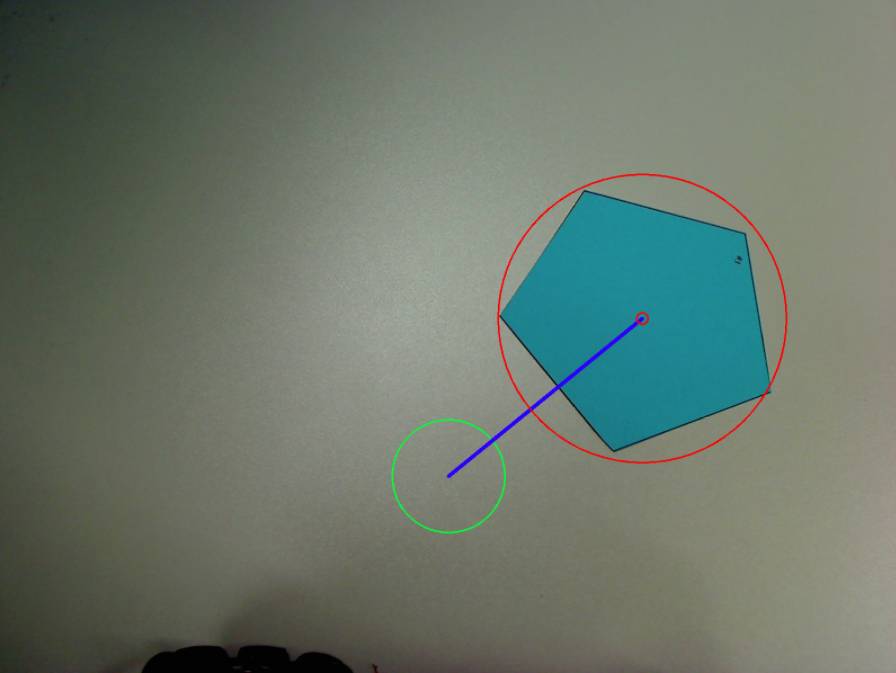
\includegraphics[width=0.4\textwidth]{fig/alignementtresor.png}
   \caption{Traitement fait lors de l'alignement avec l'ile}
   \label{f:alignement_ile}
\end{figure}


\subsection{Recharge du condensateur}
La phase d'alignement avec la station de recharge est une �tape cruciale dans le d�roulement de la routine. En effet, un mauvais alignement aura comme cons�quence un plus long temps de recharge ou aucune recharge dans le pire des cas. Il est donc indispensable que le robot soit parfaitement align� avec la station de recharge afin que la recharge � induction soit optimale. 
\medbreak
Lorsque le robot est men� � la station de recharge � l'aide de la station de base, celle-ci enverra une commande d'alignement au robot. La cam�ra se positionne face � la station de recharge et analyse la position d'une forme cible, qui se trouve au dessus de la bobine d'induction. Suite � l'analyse de l'image, l'aire de cette forme est compar�e � une aire de r�f�rence �tablie � une distance connue, la distance entre le robot et la station de base est calcul�e. Un ajustement lat�ral est aussi calcul� selon la position du centre de la forme cible. 
\medbreak
Pr�c�dant l'ex�cution des ajustements, la charge du condensateur est activ�e. La tension du condensateur est monitor�e tout au long de la recharge, car d�s que celle-ci d�passe 4.7V, on d�sactive la charge du condensateur et le robot se s�pare par la suite du la station de recharge.
\medbreak
\textit{Suite � une modification de la station de recharge, l'impl�mentation du traitement visuel n'est que partiellement cod�. Toutefois, les m�thodes expliqu�es seront celles utilis�es dans l'impl�mentation.}




\chapter{Sch�mas �lectroniques}
\label{s:Schemas}





\section{Station de recharge}
\label{s:Recharge}

\begin{figure}[htp]
   \centering
   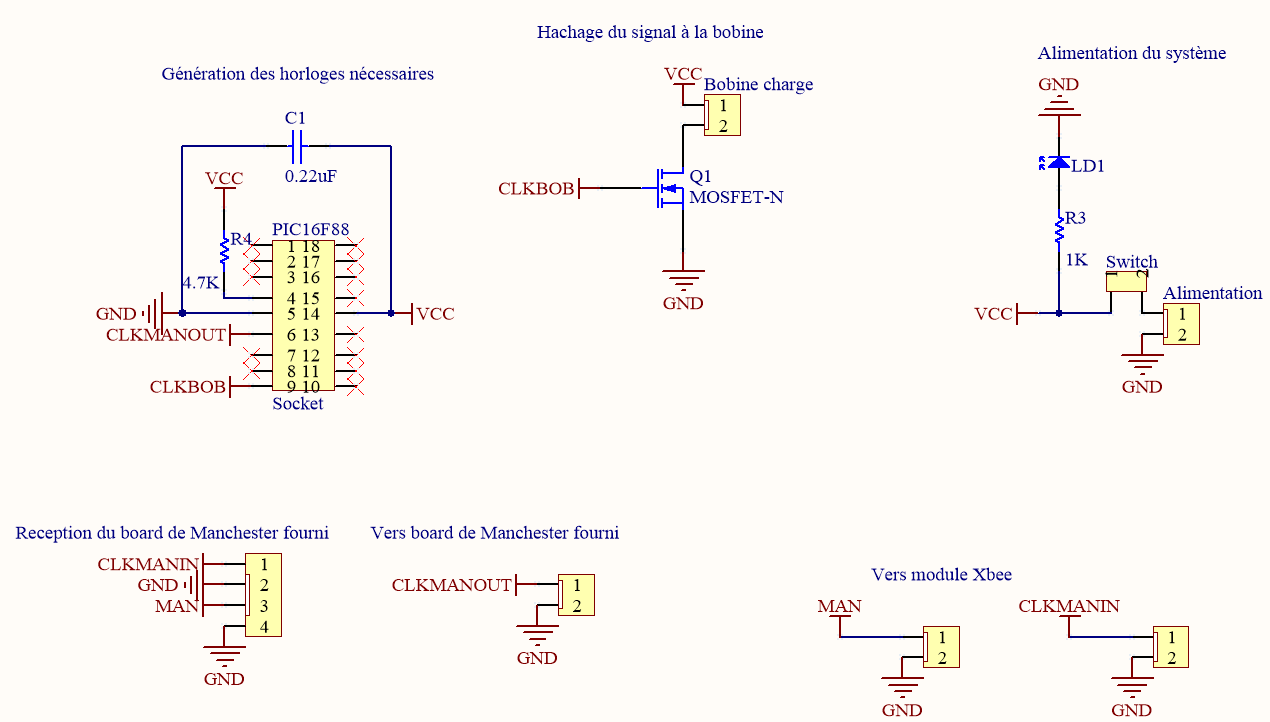
\includegraphics[width=1\textwidth]{fig/StationRecharge.png}
   \caption{Sch�ma �lectrique de la station de recharge}
   \label{f:StationRecharge}
\end{figure}


\section{Circuit de charge et de d�charge du condensateur}
\label{s:Condensateur}

\begin{figure}[htp]
   \centering
   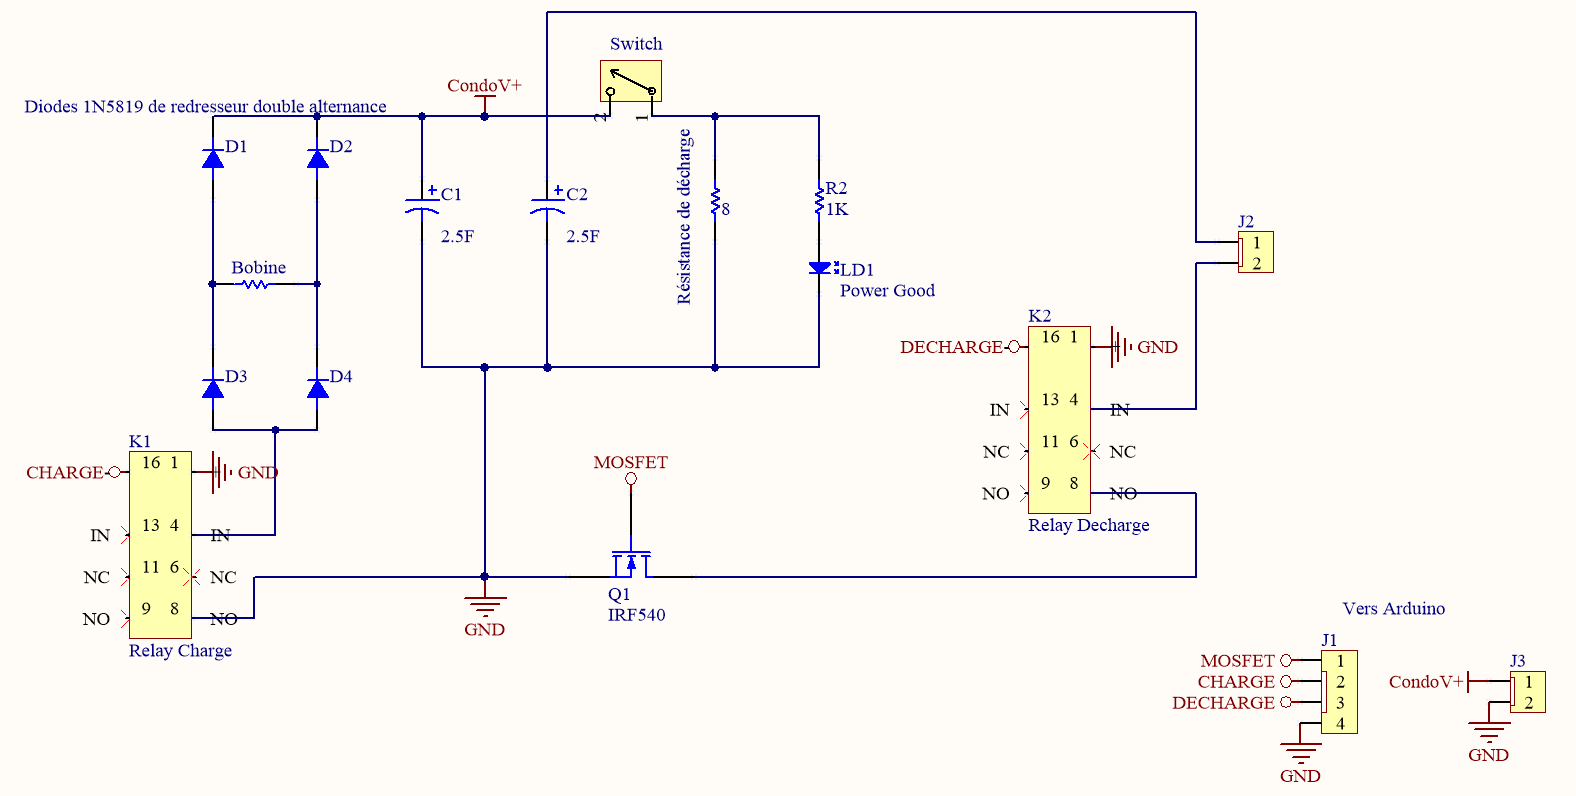
\includegraphics[width=1\textwidth]{fig/Condensateur.png}
   \caption{Sch�ma �lectrique de la charge et la d�charge du condensateur}
   \label{f:Condensateur}
\end{figure}



\section{Circuit de connections pour les moteurs}
\label{Connections}

\subsection{Connections moteurs et pont en H}
\label{Moteurs}

\begin{figure}[htp]
   \centering
   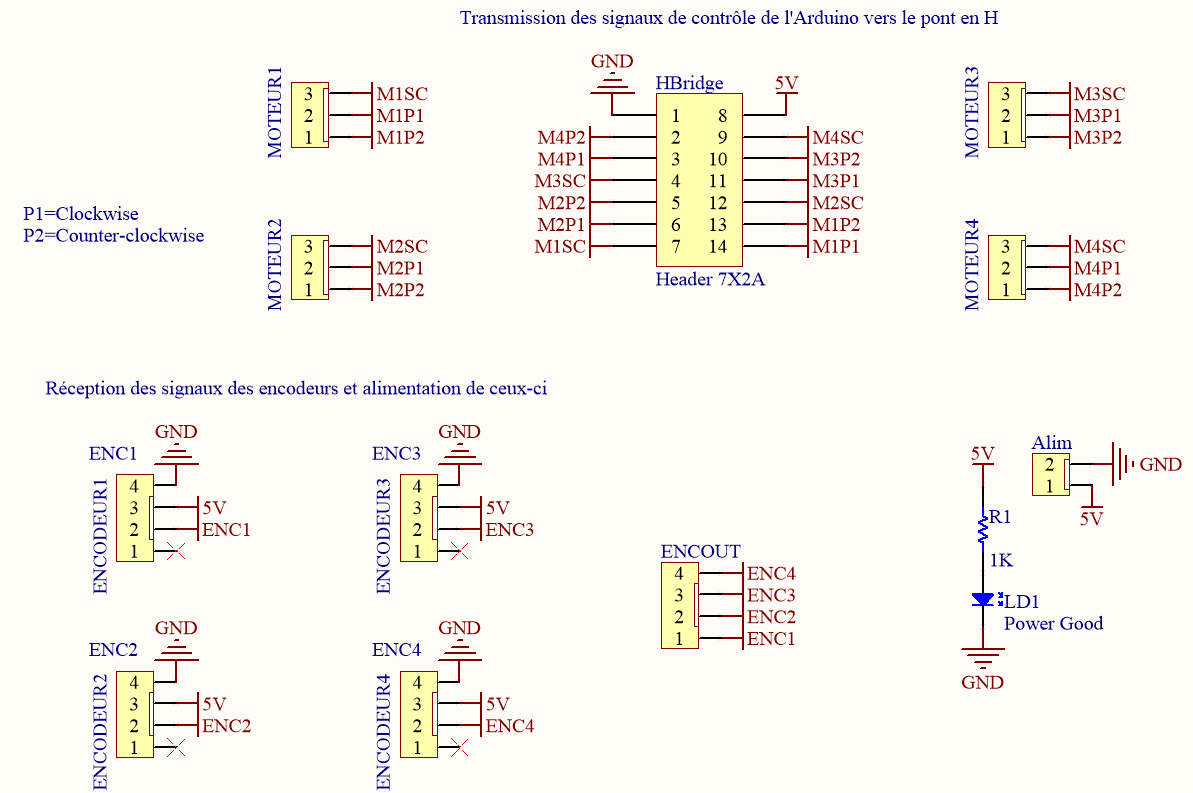
\includegraphics[width=1\textwidth]{fig/Connections.png}
   \caption{Sch�ma �lectrique du circuit de connections des moteurs}
   \label{f:Connections}
\end{figure}



\subsection{Connections sur l'Arduino}
\label{Arduino}








\section{Circuit d'alimentation}
\label{s:Alimentation}

La figure \ref{f:Alimentation} pr�sente le circuit d'alimentation utilis� sur le robot.

\begin{figure}[htp]
   \centering
   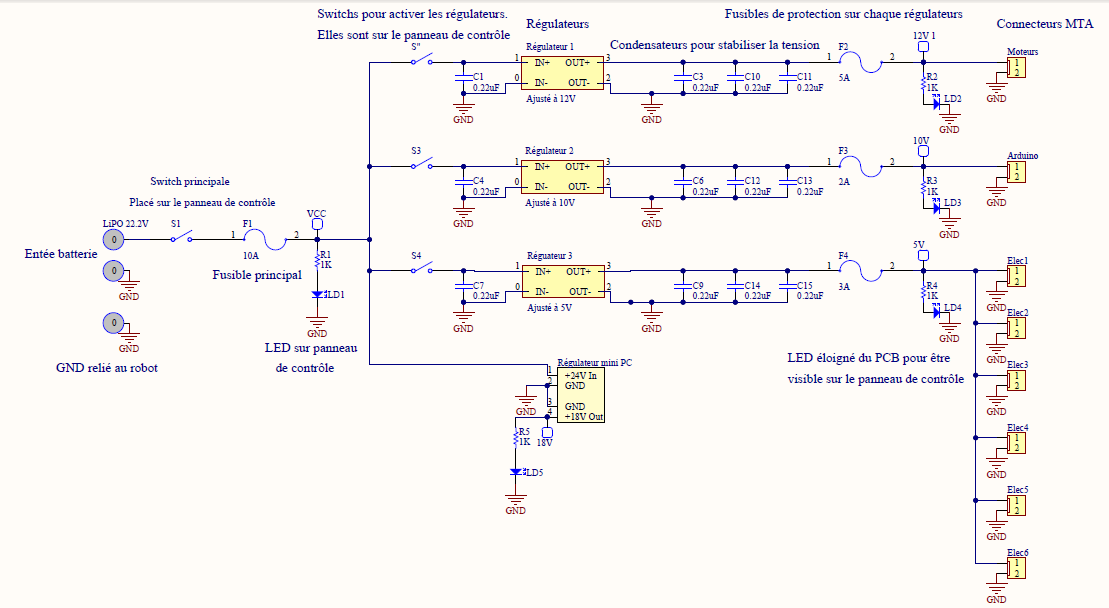
\includegraphics[width=0.85\textwidth]{fig/Alimentation.png}
   \caption{Circuit d'alimentation du robot}
   \label{f:Alimentation}
\end{figure}






%!TEX encoding = IsoLatin

%
% Chapitre "Introduction"
%

%Sites d'achats, factures, etc


\begin{thebibliographyUL}{99} % remplacer le "{9}" par "{99}" lorsque le nombre de references
                              % requiert 2 caracteres (>= 10 references)
\bibitem{MOD00} Design II (mod�lisation), \textit{Actionneur �lectromagn�tique Partie 2}, [En ligne], \url{http://wcours.gel.ulaval.ca/2015/h/GEL2007/default/5notes/Seminaire_Actionneur_Balance_2015_part2fin.pdf}, Page consult�e le 17 f�vrier 2015

\end{thebibliographyUL}

\appendix
%%!TEX encoding = IsoLatin

%
% Annexe "Liste des sigles et des acronymes"
%

\chapter{Liste des sigles et des acronymes}
\label{Sigles}

\begin{flushleft}
   \begin{tabular}{@{}ll}
      \textbf{CAO}        & Conception Assist�e par Ordinateur \\
   \end{tabular}
\end{flushleft}



\end{document}          
